L'inflazione risolve il pb e PREDICO omega=1, Plank lo misura
curvo-> piatto perché infl lo stira tantissimooooo

pot chimico dice come l'energia interna reagisce ad una variazione di densità
omega b storicamente con fotoni galassie, poi nucleosintesiii

\begin{equation}
    \left\{\begin{matrix}
        t^{1/s} & -1 < w \le 1/3\\ 
        (cost-t)^{1/s} & w<-1 \\
        \exp (t/\tau)&  w=-1
       \end{matrix}\right.
\end{equation}

\begin{equation}\left\{
    \def\arraystretch{1.5}
        \begin{array}{ll}
        T_P \simeq 10^{32}~\mathrm{K} \\
        E_P \simeq 10^{19}~\mathrm{Gev} \\
        n_P \simeq 10^{98}~\mathrm{cm}^{-3} \\
        m_P \simeq 10^{-5}~\mathrm{g} \\
        \rho_P \simeq 10^{93}~\mathrm{g\: cm}^{-3}  \\
        l_P \simeq 10^{-33}~\mathrm{cm} \\
        \sigma = (entropia) = 1 
    \end{array}\right. \label{eq:unitaplanckiane}
\end{equation}


\begin{figure}[H]
    \centering
    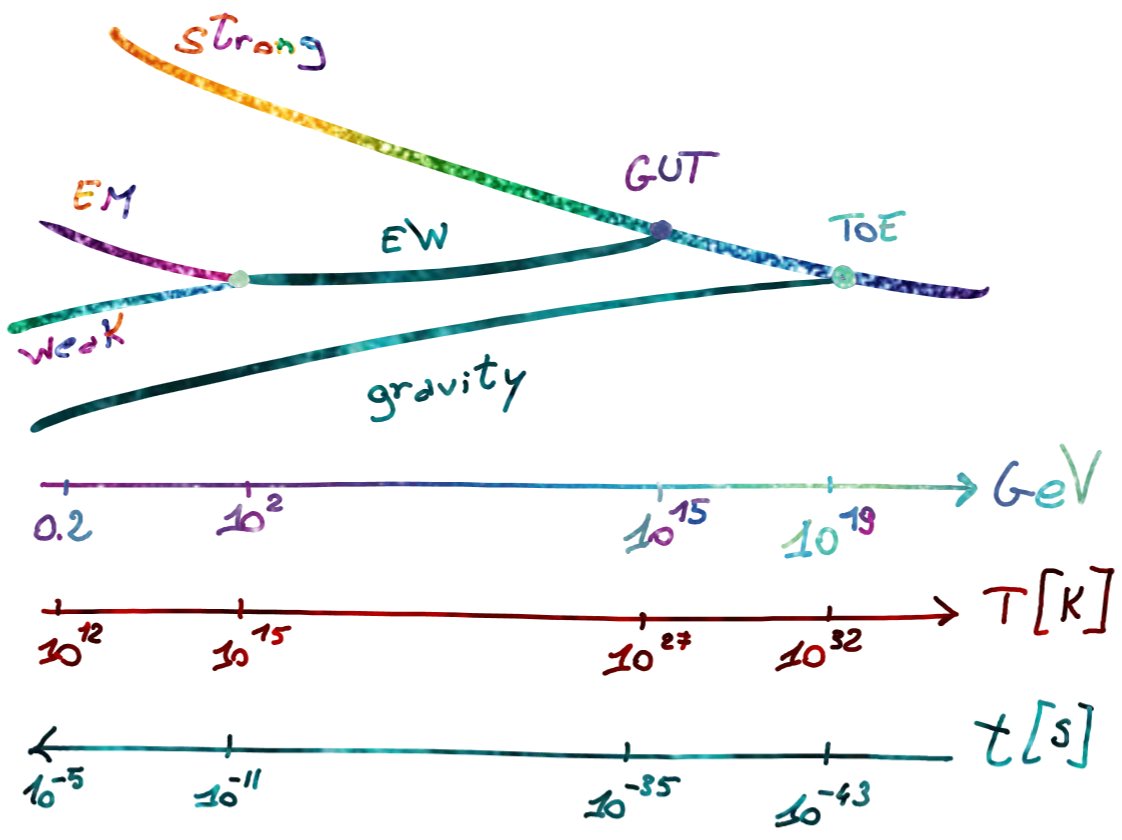
\includegraphics[width=.55 \textwidth]{Pictures/5/fasiprimordiali.png}
    \caption{fig:4}
\end{figure}

\begin{figure}[H]
    \subfloat[]{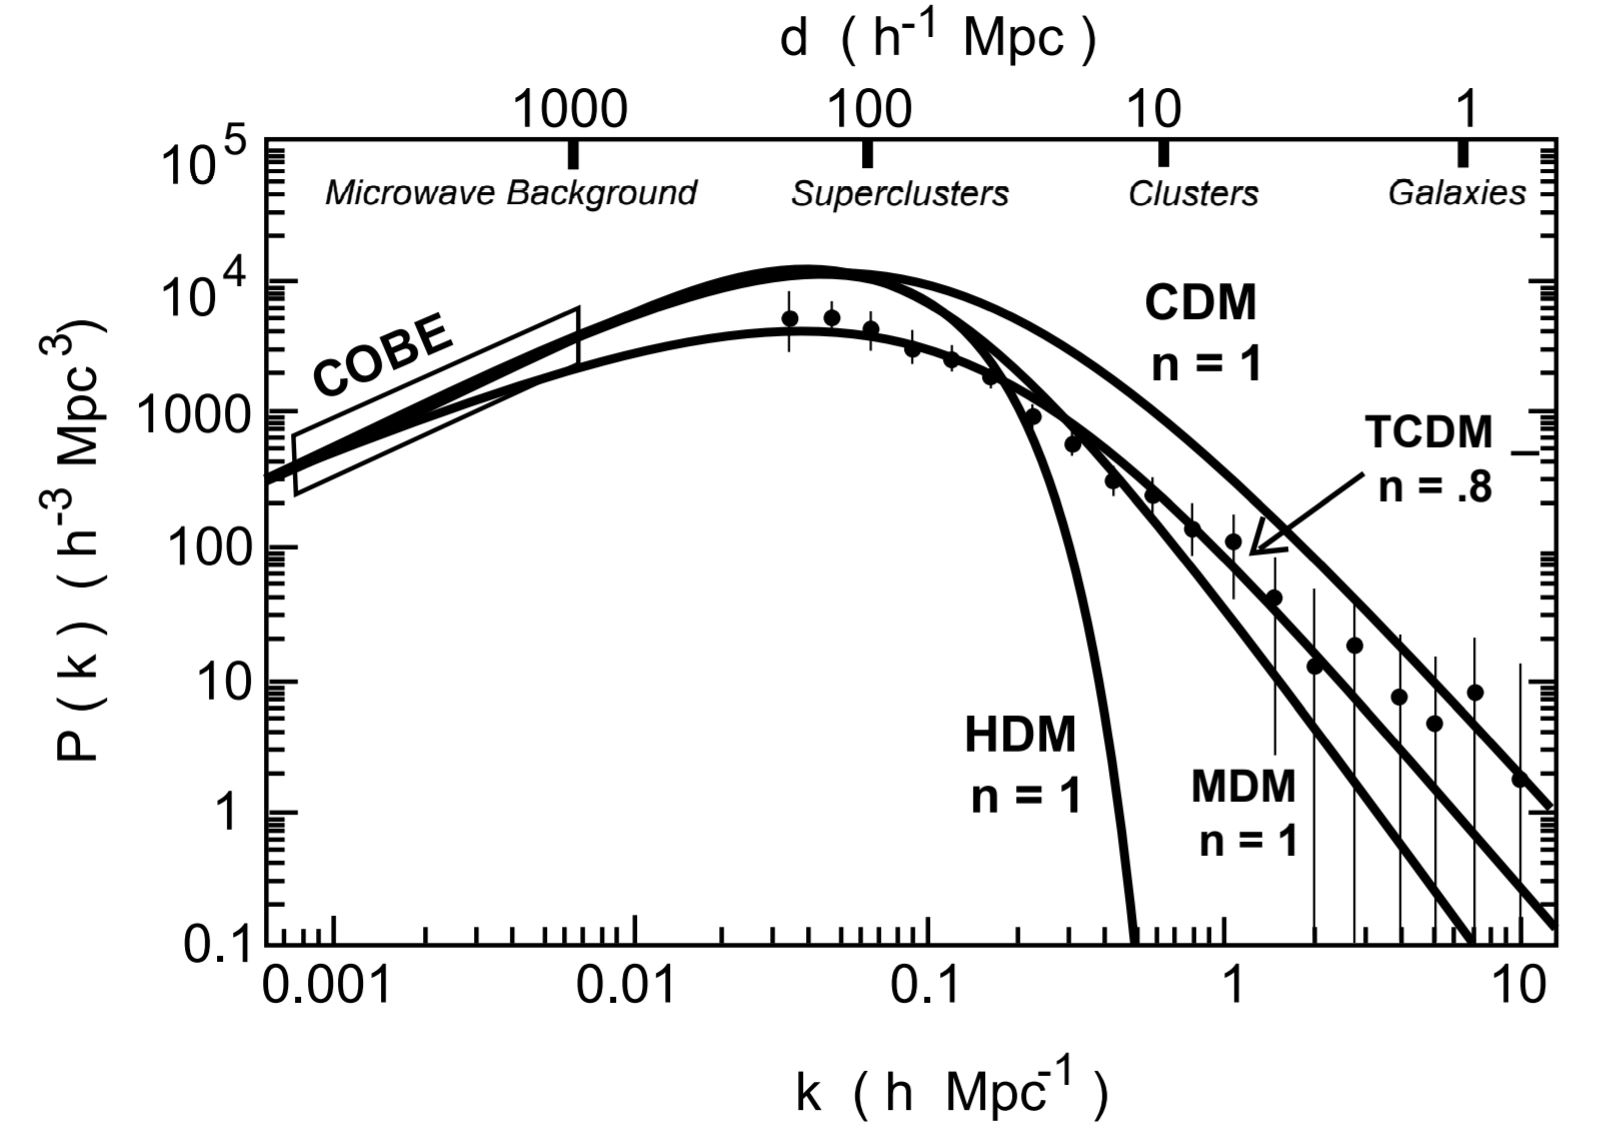
\includegraphics[width=.6\textwidth]{Pictures/8/tris1.jpg}}$\;\;$
    \subfloat[]{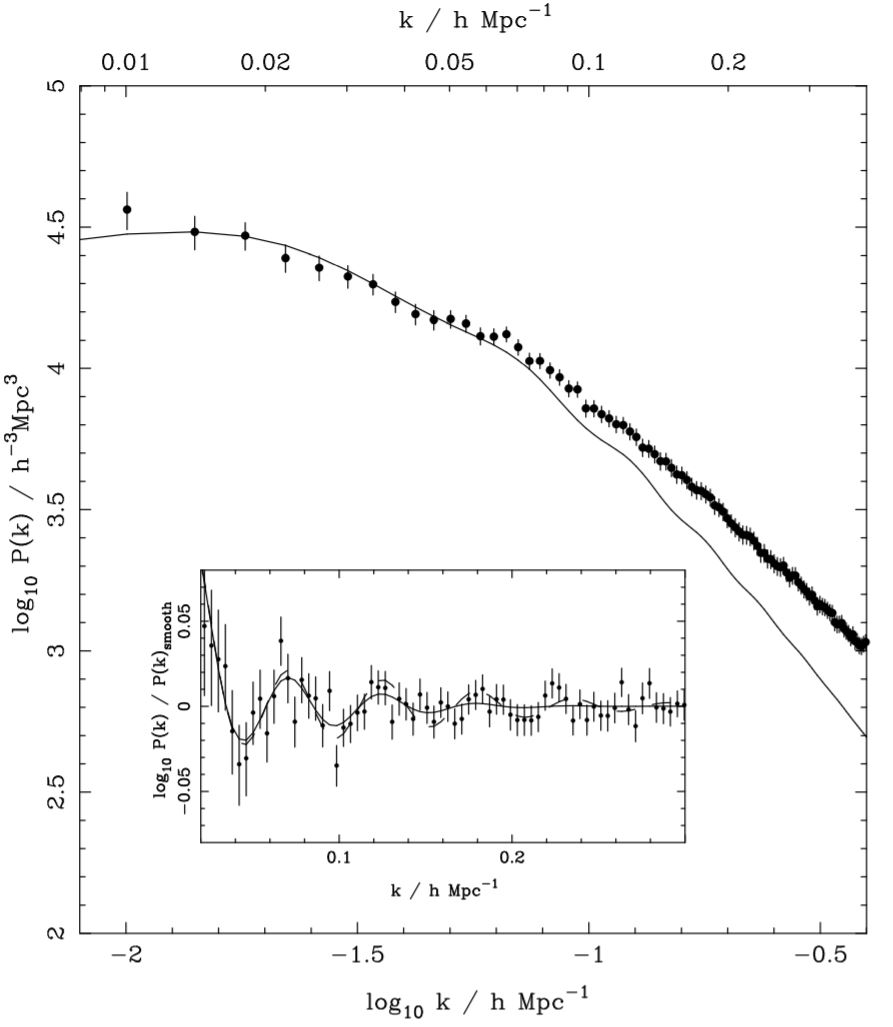
\includegraphics[width=.355\textwidth]{Pictures/8/tris3.jpg}}
    \caption{(a) Modelli di densità di potenza per Hot, Mixed (Warm) e Cold Dark Matter (i punti rappresentano i dati osservati che fittano un modello \textit{tilted}) (From: Kolb - \textit{Particle Physics in the Early Universe}, 1998); (b) Redshift-space power spectrum (notare $k/h$ sulle ascisse) per un campione di galassie (From: Percival et al. - \textit{The shape of the SDSS DR5 galaxy power spectrum}, 2006).} \label{fig8:bella3} 
\end{figure}


\hslash
\mathcal{P}(k)

\begin{example}[Materia non relativistica]
$p_m=nk_B T = \frac{\rho_m}{m_p}k_B T \approx 0 \qquad ( \rho_m \approx 0) $
\end{example}
\begin{example}[Radiazione o Materia relativistica]
$p_R=\frac{1}{3} \rho_R c^2 $
\end{example}
\begin{example}[Costante Cosmologica]
$p_\Lambda= -\rho_\Lambda c^2 $
\end{example}



È

Single quotation marks are produced in LaTeX using ` and ' . Double quotation marks are produced by typing `` and '' .



ERA DELLA MATERIA 3000-6000 (dominante rispetto radiazione)  dall'equivalenza a oggi (anche se oggi lambda).
Andamento Grho nelle lambda jeans

La velocità è sempre più lineare del campo di densità (ha dei k in meno)


che tradotto in termini di spettro del potenziale diventa
P(k) / kn􀀀1 = k0 = cost